Each APA is instrumented with 20 Front End Mother Boards (FEMBs).
The FEMBs plug into the APA CR boards, making the connections from the wires to the charge amplifier circuits as short as possible.
Each FEMB receives signals from 40 U wires, 40 V wires, and 48 X wires.
The baseline FEMB design contains 8 16-channel Front-End (LArASIC) ASICs, 8 16-channel Cold ADC ASICs, and 2 COLDATA control and communication ASICs (see Figure~\ref{fig:ce-scheme}).
The FEMB also contains regulators which produce the voltages required by the ASICs and 
filter those voltages.
The LArASIC inputs are protected by diodes and a series inductor.

\begin{dunefigure}
[The baseline CE architecture. The basic unit is the 128-channel FEMB. Note that only one CE flange is shown to simplify the illustration.]
{fig:ce-scheme}
{The baseline CE architecture. The basic unit is the 128-channel FEMB. Note that only one CE flange is shown to simplify the illustration.}
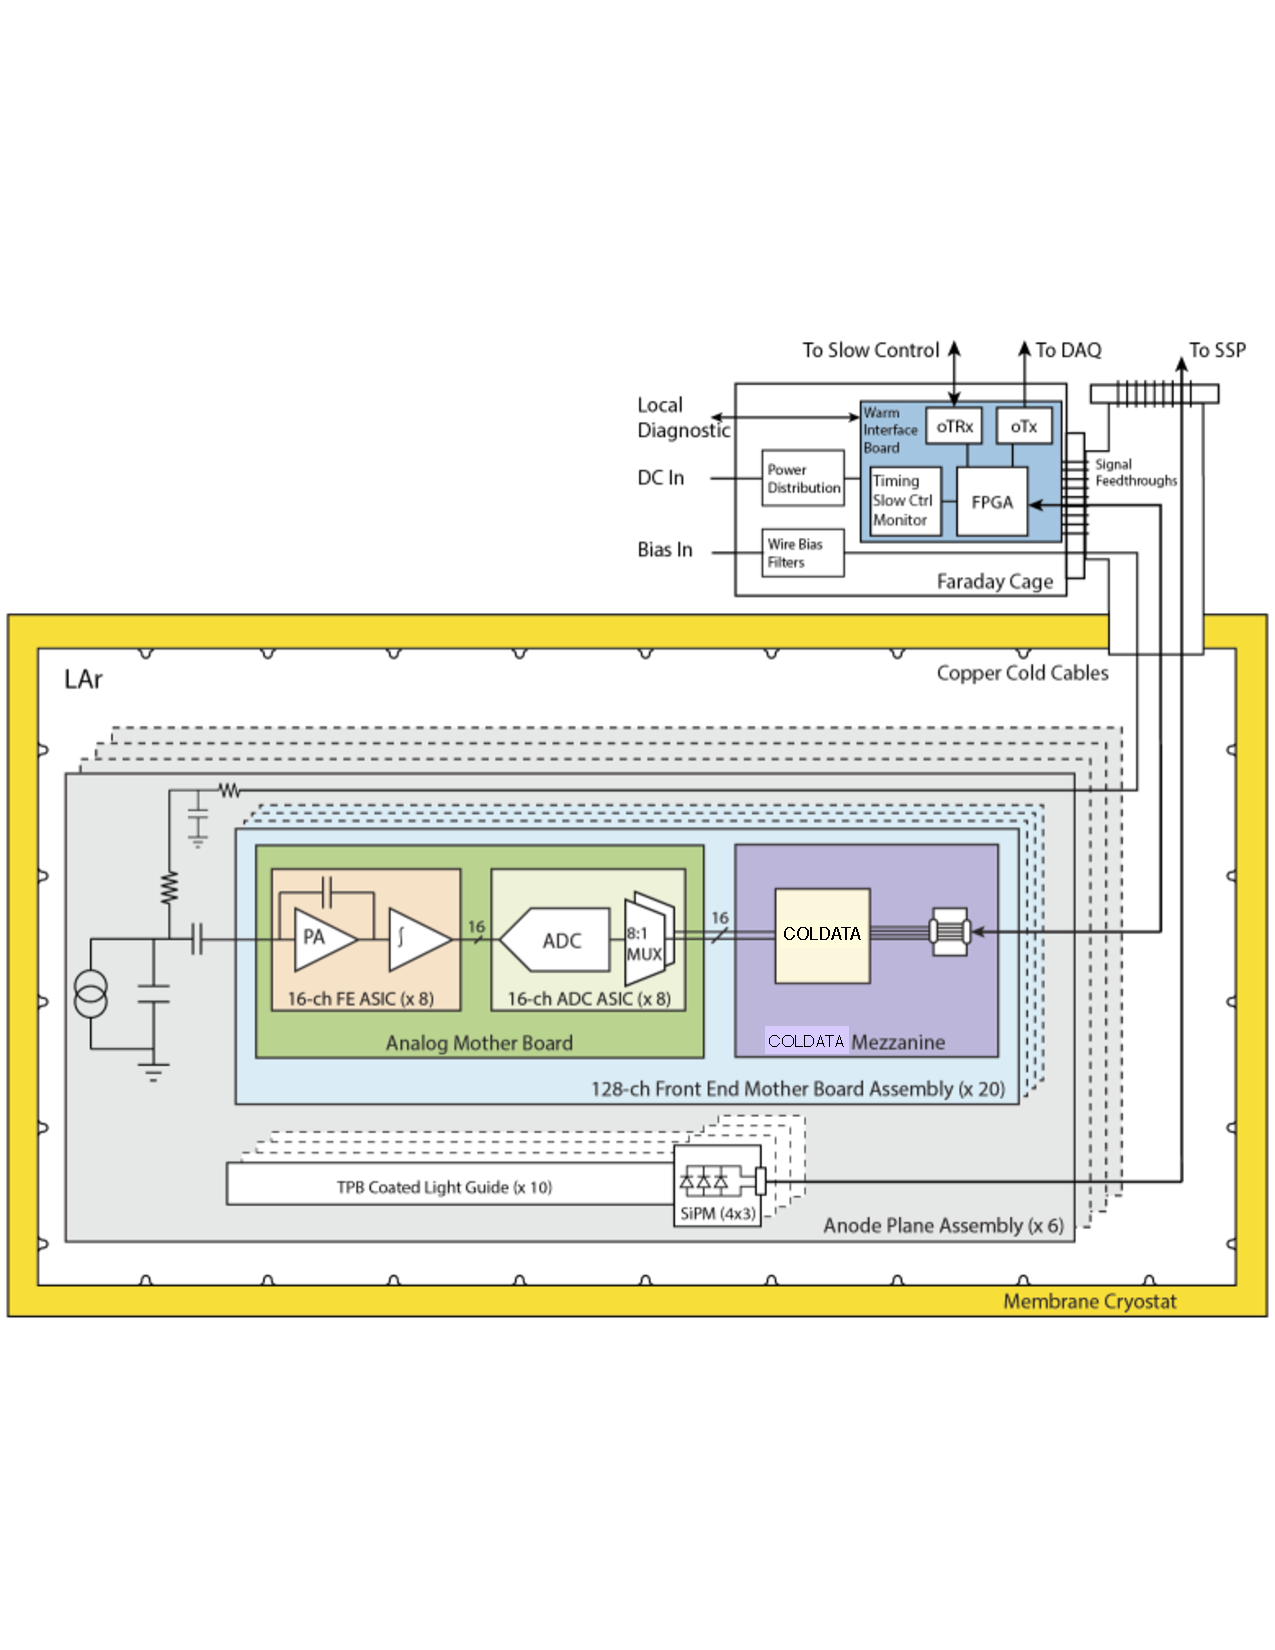
\includegraphics[width=0.9\linewidth]{tpcelec-schem_v2.pdf}
\end{dunefigure}

The ProtoDUNE-SP version of the FEMB (which uses a single FPGA on a mezzanine card instead of two COLDATA ASICs) is shown in Figure~\ref{fig:femb}.

\begin{dunefigure}
[The complete FEMB assembly as used in the ProtoDUNE-SP detector. The cable shown is the high-speed data, clock, and control cable.]
{fig:femb}
{The complete FEMB assembly as used in the ProtoDUNE-SP detector. The cable shown is the high-speed data, clock, and control cable.}
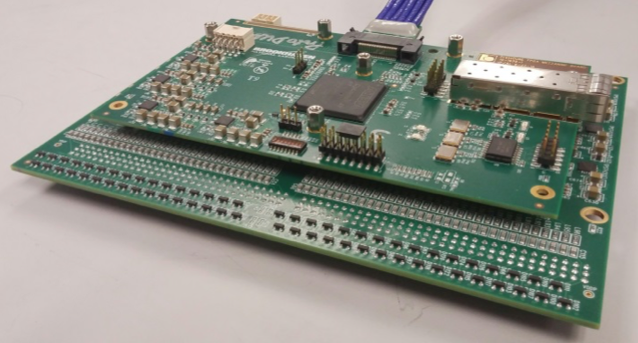
\includegraphics[width=0.6\linewidth]{tpcelec-femb.png}
\end{dunefigure}
